% Options for packages loaded elsewhere
\PassOptionsToPackage{unicode}{hyperref}
\PassOptionsToPackage{hyphens}{url}
\documentclass[
]{article}
\usepackage{xcolor}
\usepackage[margin=1in]{geometry}
\usepackage{amsmath,amssymb}
\setcounter{secnumdepth}{5}
\usepackage{iftex}
\ifPDFTeX
  \usepackage[T1]{fontenc}
  \usepackage[utf8]{inputenc}
  \usepackage{textcomp} % provide euro and other symbols
\else % if luatex or xetex
  \usepackage{unicode-math} % this also loads fontspec
  \defaultfontfeatures{Scale=MatchLowercase}
  \defaultfontfeatures[\rmfamily]{Ligatures=TeX,Scale=1}
\fi
\usepackage{lmodern}
\ifPDFTeX\else
  % xetex/luatex font selection
\fi
% Use upquote if available, for straight quotes in verbatim environments
\IfFileExists{upquote.sty}{\usepackage{upquote}}{}
\IfFileExists{microtype.sty}{% use microtype if available
  \usepackage[]{microtype}
  \UseMicrotypeSet[protrusion]{basicmath} % disable protrusion for tt fonts
}{}
\makeatletter
\@ifundefined{KOMAClassName}{% if non-KOMA class
  \IfFileExists{parskip.sty}{%
    \usepackage{parskip}
  }{% else
    \setlength{\parindent}{0pt}
    \setlength{\parskip}{6pt plus 2pt minus 1pt}}
}{% if KOMA class
  \KOMAoptions{parskip=half}}
\makeatother
\usepackage{color}
\usepackage{fancyvrb}
\newcommand{\VerbBar}{|}
\newcommand{\VERB}{\Verb[commandchars=\\\{\}]}
\DefineVerbatimEnvironment{Highlighting}{Verbatim}{commandchars=\\\{\}}
% Add ',fontsize=\small' for more characters per line
\usepackage{framed}
\definecolor{shadecolor}{RGB}{248,248,248}
\newenvironment{Shaded}{\begin{snugshade}}{\end{snugshade}}
\newcommand{\AlertTok}[1]{\textcolor[rgb]{0.94,0.16,0.16}{#1}}
\newcommand{\AnnotationTok}[1]{\textcolor[rgb]{0.56,0.35,0.01}{\textbf{\textit{#1}}}}
\newcommand{\AttributeTok}[1]{\textcolor[rgb]{0.13,0.29,0.53}{#1}}
\newcommand{\BaseNTok}[1]{\textcolor[rgb]{0.00,0.00,0.81}{#1}}
\newcommand{\BuiltInTok}[1]{#1}
\newcommand{\CharTok}[1]{\textcolor[rgb]{0.31,0.60,0.02}{#1}}
\newcommand{\CommentTok}[1]{\textcolor[rgb]{0.56,0.35,0.01}{\textit{#1}}}
\newcommand{\CommentVarTok}[1]{\textcolor[rgb]{0.56,0.35,0.01}{\textbf{\textit{#1}}}}
\newcommand{\ConstantTok}[1]{\textcolor[rgb]{0.56,0.35,0.01}{#1}}
\newcommand{\ControlFlowTok}[1]{\textcolor[rgb]{0.13,0.29,0.53}{\textbf{#1}}}
\newcommand{\DataTypeTok}[1]{\textcolor[rgb]{0.13,0.29,0.53}{#1}}
\newcommand{\DecValTok}[1]{\textcolor[rgb]{0.00,0.00,0.81}{#1}}
\newcommand{\DocumentationTok}[1]{\textcolor[rgb]{0.56,0.35,0.01}{\textbf{\textit{#1}}}}
\newcommand{\ErrorTok}[1]{\textcolor[rgb]{0.64,0.00,0.00}{\textbf{#1}}}
\newcommand{\ExtensionTok}[1]{#1}
\newcommand{\FloatTok}[1]{\textcolor[rgb]{0.00,0.00,0.81}{#1}}
\newcommand{\FunctionTok}[1]{\textcolor[rgb]{0.13,0.29,0.53}{\textbf{#1}}}
\newcommand{\ImportTok}[1]{#1}
\newcommand{\InformationTok}[1]{\textcolor[rgb]{0.56,0.35,0.01}{\textbf{\textit{#1}}}}
\newcommand{\KeywordTok}[1]{\textcolor[rgb]{0.13,0.29,0.53}{\textbf{#1}}}
\newcommand{\NormalTok}[1]{#1}
\newcommand{\OperatorTok}[1]{\textcolor[rgb]{0.81,0.36,0.00}{\textbf{#1}}}
\newcommand{\OtherTok}[1]{\textcolor[rgb]{0.56,0.35,0.01}{#1}}
\newcommand{\PreprocessorTok}[1]{\textcolor[rgb]{0.56,0.35,0.01}{\textit{#1}}}
\newcommand{\RegionMarkerTok}[1]{#1}
\newcommand{\SpecialCharTok}[1]{\textcolor[rgb]{0.81,0.36,0.00}{\textbf{#1}}}
\newcommand{\SpecialStringTok}[1]{\textcolor[rgb]{0.31,0.60,0.02}{#1}}
\newcommand{\StringTok}[1]{\textcolor[rgb]{0.31,0.60,0.02}{#1}}
\newcommand{\VariableTok}[1]{\textcolor[rgb]{0.00,0.00,0.00}{#1}}
\newcommand{\VerbatimStringTok}[1]{\textcolor[rgb]{0.31,0.60,0.02}{#1}}
\newcommand{\WarningTok}[1]{\textcolor[rgb]{0.56,0.35,0.01}{\textbf{\textit{#1}}}}
\usepackage{longtable,booktabs,array}
\usepackage{calc} % for calculating minipage widths
% Correct order of tables after \paragraph or \subparagraph
\usepackage{etoolbox}
\makeatletter
\patchcmd\longtable{\par}{\if@noskipsec\mbox{}\fi\par}{}{}
\makeatother
% Allow footnotes in longtable head/foot
\IfFileExists{footnotehyper.sty}{\usepackage{footnotehyper}}{\usepackage{footnote}}
\makesavenoteenv{longtable}
\usepackage{graphicx}
\makeatletter
\newsavebox\pandoc@box
\newcommand*\pandocbounded[1]{% scales image to fit in text height/width
  \sbox\pandoc@box{#1}%
  \Gscale@div\@tempa{\textheight}{\dimexpr\ht\pandoc@box+\dp\pandoc@box\relax}%
  \Gscale@div\@tempb{\linewidth}{\wd\pandoc@box}%
  \ifdim\@tempb\p@<\@tempa\p@\let\@tempa\@tempb\fi% select the smaller of both
  \ifdim\@tempa\p@<\p@\scalebox{\@tempa}{\usebox\pandoc@box}%
  \else\usebox{\pandoc@box}%
  \fi%
}
% Set default figure placement to htbp
\def\fps@figure{htbp}
\makeatother
\setlength{\emergencystretch}{3em} % prevent overfull lines
\providecommand{\tightlist}{%
  \setlength{\itemsep}{0pt}\setlength{\parskip}{0pt}}
\usepackage[]{natbib}
\bibliographystyle{plainnat}
\usepackage{bookmark}
\IfFileExists{xurl.sty}{\usepackage{xurl}}{} % add URL line breaks if available
\urlstyle{same}
\hypersetup{
  pdftitle={Appendix A --- Summary Analytics: Lichess vs.~FIDE Rating Patterns},
  pdfauthor={Tina Huynh},
  hidelinks,
  pdfcreator={LaTeX via pandoc}}

\title{Appendix A --- Summary Analytics: Lichess vs.~FIDE Rating
Patterns}
\author{Tina Huynh}
\date{2025-10-16}

\begin{document}
\maketitle

{
\setcounter{tocdepth}{2}
\tableofcontents
}
\subsection{Appendix A --- Summary Analytics: Lichess vs.~FIDE Rating
Patterns}\label{appendix-a-summary-analytics-lichess-vs.-fide-rating-patterns}

\subsubsection{A.1 Data Import and
Preparation}\label{a.1-data-import-and-preparation}

\begin{Shaded}
\begin{Highlighting}[]
\FunctionTok{library}\NormalTok{(tidyverse)}
\FunctionTok{library}\NormalTok{(scales)}

\CommentTok{\# Define correct paths relative to repo structure}
\NormalTok{summary\_path }\OtherTok{\textless{}{-}} \StringTok{"../../data/player\_summary.csv"}

\CommentTok{\# Import the summary dataset generated by data\_import.R}
\NormalTok{player\_summary }\OtherTok{\textless{}{-}} \FunctionTok{read\_csv}\NormalTok{(summary\_path, }\AttributeTok{show\_col\_types =} \ConstantTok{FALSE}\NormalTok{)}

\CommentTok{\# Verify import and inspect structure}
\FunctionTok{glimpse}\NormalTok{(player\_summary)}
\end{Highlighting}
\end{Shaded}

\begin{verbatim}
## Rows: 5
## Columns: 25
## $ rating_group              <chr> "1600–1999", "2000–2399", "2400–2599", "2600~
## $ lichess_players           <dbl> 60, 129, 93, 207, 38
## $ lichess_avg_rating        <dbl> 1815.5, 2240.9, 2504.3, 2867.6, 1383.8
## $ lichess_rating_sd         <dbl> 122.4, 109.7, 58.3, 177.8, 154.7
## $ lichess_avg_games         <dbl> 14.6, 14.9, 15.0, 15.0, 12.3
## $ lichess_avg_win_rate      <dbl> 0.553, 0.620, 0.619, 0.665, 0.449
## $ lichess_avg_rating_change <dbl> 9.07, 3.07, 0.26, 0.53, -13.91
## $ pct_high_activity         <dbl> 0, 0, 0, 0, 0
## $ avg_days_active           <dbl> 151.7, 46.0, 26.0, 16.4, 125.2
## $ pct_prefer_blitz          <dbl> 0.400, 0.388, 0.398, 0.319, 0.316
## $ pct_prefer_rapid          <dbl> 0.067, 0.109, 0.129, 0.048, 0.184
## $ pct_prefer_bullet         <dbl> 0.483, 0.403, 0.409, 0.628, 0.447
## $ fide_players              <dbl> 285, 238, 76, 19, 332
## $ fide_avg_rating_standard  <dbl> 1805.5, 2208.2, 2487.9, 2872.5, 1207.3
## $ fide_avg_rating_blitz     <dbl> 1778.4, 2186.8, 2461.3, 2804.5, 1180.5
## $ fide_rating_sd            <dbl> 115.4, 117.1, 56.1, 187.0, 217.7
## $ fide_avg_games            <dbl> 54.4, 55.0, 85.3, 129.9, 53.1
## $ fide_pct_titled           <dbl> 0.144, 0.416, 0.711, 0.842, 0.127
## $ fide_pct_active           <dbl> 0.761, 0.773, 0.842, 0.842, 0.744
## $ fide_avg_age              <dbl> 44.6, 47.7, 43.8, 45.6, 46.0
## $ total_players             <dbl> 345, 367, 169, 226, 370
## $ rating_gap_standard       <dbl> 10.0, 32.7, 16.4, -4.9, 176.5
## $ rating_gap_blitz          <dbl> 37.1, 54.1, 43.0, 63.1, 203.3
## $ activity_ratio            <dbl> 0.27, 0.27, 0.18, 0.12, 0.23
## $ platform_preference       <chr> "Balanced", "Balanced", "Online Preferred", ~
\end{verbatim}

\begin{Shaded}
\begin{Highlighting}[]
\FunctionTok{summary}\NormalTok{(player\_summary)}
\end{Highlighting}
\end{Shaded}

\begin{verbatim}
##  rating_group       lichess_players lichess_avg_rating lichess_rating_sd
##  Length:5           Min.   : 38.0   Min.   :1384       Min.   : 58.3    
##  Class :character   1st Qu.: 60.0   1st Qu.:1816       1st Qu.:109.7    
##  Mode  :character   Median : 93.0   Median :2241       Median :122.4    
##                     Mean   :105.4   Mean   :2162       Mean   :124.6    
##                     3rd Qu.:129.0   3rd Qu.:2504       3rd Qu.:154.7    
##                     Max.   :207.0   Max.   :2868       Max.   :177.8    
##  lichess_avg_games lichess_avg_win_rate lichess_avg_rating_change
##  Min.   :12.30     Min.   :0.4490       Min.   :-13.910          
##  1st Qu.:14.60     1st Qu.:0.5530       1st Qu.:  0.260          
##  Median :14.90     Median :0.6190       Median :  0.530          
##  Mean   :14.36     Mean   :0.5812       Mean   : -0.196          
##  3rd Qu.:15.00     3rd Qu.:0.6200       3rd Qu.:  3.070          
##  Max.   :15.00     Max.   :0.6650       Max.   :  9.070          
##  pct_high_activity avg_days_active  pct_prefer_blitz pct_prefer_rapid
##  Min.   :0         Min.   : 16.40   Min.   :0.3160   Min.   :0.0480  
##  1st Qu.:0         1st Qu.: 26.00   1st Qu.:0.3190   1st Qu.:0.0670  
##  Median :0         Median : 46.00   Median :0.3880   Median :0.1090  
##  Mean   :0         Mean   : 73.06   Mean   :0.3642   Mean   :0.1074  
##  3rd Qu.:0         3rd Qu.:125.20   3rd Qu.:0.3980   3rd Qu.:0.1290  
##  Max.   :0         Max.   :151.70   Max.   :0.4000   Max.   :0.1840  
##  pct_prefer_bullet  fide_players fide_avg_rating_standard fide_avg_rating_blitz
##  Min.   :0.403     Min.   : 19   Min.   :1207             Min.   :1180         
##  1st Qu.:0.409     1st Qu.: 76   1st Qu.:1806             1st Qu.:1778         
##  Median :0.447     Median :238   Median :2208             Median :2187         
##  Mean   :0.474     Mean   :190   Mean   :2116             Mean   :2082         
##  3rd Qu.:0.483     3rd Qu.:285   3rd Qu.:2488             3rd Qu.:2461         
##  Max.   :0.628     Max.   :332   Max.   :2872             Max.   :2804         
##  fide_rating_sd  fide_avg_games   fide_pct_titled fide_pct_active 
##  Min.   : 56.1   Min.   : 53.10   Min.   :0.127   Min.   :0.7440  
##  1st Qu.:115.4   1st Qu.: 54.40   1st Qu.:0.144   1st Qu.:0.7610  
##  Median :117.1   Median : 55.00   Median :0.416   Median :0.7730  
##  Mean   :138.7   Mean   : 75.54   Mean   :0.448   Mean   :0.7924  
##  3rd Qu.:187.0   3rd Qu.: 85.30   3rd Qu.:0.711   3rd Qu.:0.8420  
##  Max.   :217.7   Max.   :129.90   Max.   :0.842   Max.   :0.8420  
##   fide_avg_age   total_players   rating_gap_standard rating_gap_blitz
##  Min.   :43.80   Min.   :169.0   Min.   : -4.90      Min.   : 37.10  
##  1st Qu.:44.60   1st Qu.:226.0   1st Qu.: 10.00      1st Qu.: 43.00  
##  Median :45.60   Median :345.0   Median : 16.40      Median : 54.10  
##  Mean   :45.54   Mean   :295.4   Mean   : 46.14      Mean   : 80.12  
##  3rd Qu.:46.00   3rd Qu.:367.0   3rd Qu.: 32.70      3rd Qu.: 63.10  
##  Max.   :47.70   Max.   :370.0   Max.   :176.50      Max.   :203.30  
##  activity_ratio  platform_preference
##  Min.   :0.120   Length:5           
##  1st Qu.:0.180   Class :character   
##  Median :0.230   Mode  :character   
##  Mean   :0.214                      
##  3rd Qu.:0.270                      
##  Max.   :0.270
\end{verbatim}

\begin{center}\rule{0.5\linewidth}{0.5pt}\end{center}

\subsubsection{A.2 Descriptive Overview}\label{a.2-descriptive-overview}

\begin{Shaded}
\begin{Highlighting}[]
\CommentTok{\# Summary statistics table}
\NormalTok{player\_summary }\SpecialCharTok{\%\textgreater{}\%}
  \FunctionTok{select}\NormalTok{(}
\NormalTok{    rating\_group, fide\_avg\_rating\_standard, lichess\_avg\_rating,}
\NormalTok{    lichess\_avg\_win\_rate, lichess\_avg\_rating\_change, rating\_gap\_standard,}
\NormalTok{    lichess\_players, fide\_players}
\NormalTok{  ) }\SpecialCharTok{\%\textgreater{}\%}
    \FunctionTok{mutate}\NormalTok{(}\FunctionTok{across}\NormalTok{(}\FunctionTok{where}\NormalTok{(is.numeric), round, }\DecValTok{2}\NormalTok{)) }\SpecialCharTok{\%\textgreater{}\%}
\NormalTok{    knitr}\SpecialCharTok{::}\FunctionTok{kable}\NormalTok{(}
      \AttributeTok{caption =} \StringTok{"Summary of Mean Ratings, Win Rates, and Player Counts by Rating Group"}\NormalTok{,}
      \AttributeTok{col.names =} \FunctionTok{c}\NormalTok{(}
        \StringTok{"Rating Group"}\NormalTok{, }\StringTok{"FIDE Avg"}\NormalTok{, }\StringTok{"Lichess Avg"}\NormalTok{, }\StringTok{"Win Rate"}\NormalTok{,}
        \StringTok{"Rating Change"}\NormalTok{, }\StringTok{"Gap"}\NormalTok{, }\StringTok{"Lichess N"}\NormalTok{, }\StringTok{"FIDE N"}
\NormalTok{      ),}
      \AttributeTok{align =} \FunctionTok{c}\NormalTok{(}\StringTok{"l"}\NormalTok{, }\FunctionTok{rep}\NormalTok{(}\StringTok{"r"}\NormalTok{, }\DecValTok{7}\NormalTok{))}
\NormalTok{    )}
\end{Highlighting}
\end{Shaded}

\begin{verbatim}
## Warning: There was 1 warning in `mutate()`.
## i In argument: `across(where(is.numeric), round, 2)`.
## Caused by warning:
## ! The `...` argument of `across()` is deprecated as of dplyr 1.1.0.
## Supply arguments directly to `.fns` through an anonymous function instead.
## 
##   # Previously
##   across(a:b, mean, na.rm = TRUE)
## 
##   # Now
##   across(a:b, \(x) mean(x, na.rm = TRUE))
\end{verbatim}

\begin{longtable}[]{@{}
  >{\raggedright\arraybackslash}p{(\linewidth - 14\tabcolsep) * \real{0.1625}}
  >{\raggedleft\arraybackslash}p{(\linewidth - 14\tabcolsep) * \real{0.1125}}
  >{\raggedleft\arraybackslash}p{(\linewidth - 14\tabcolsep) * \real{0.1500}}
  >{\raggedleft\arraybackslash}p{(\linewidth - 14\tabcolsep) * \real{0.1125}}
  >{\raggedleft\arraybackslash}p{(\linewidth - 14\tabcolsep) * \real{0.1750}}
  >{\raggedleft\arraybackslash}p{(\linewidth - 14\tabcolsep) * \real{0.0750}}
  >{\raggedleft\arraybackslash}p{(\linewidth - 14\tabcolsep) * \real{0.1250}}
  >{\raggedleft\arraybackslash}p{(\linewidth - 14\tabcolsep) * \real{0.0875}}@{}}
\caption{Summary of Mean Ratings, Win Rates, and Player Counts by Rating
Group}\tabularnewline
\toprule\noalign{}
\begin{minipage}[b]{\linewidth}\raggedright
Rating Group
\end{minipage} & \begin{minipage}[b]{\linewidth}\raggedleft
FIDE Avg
\end{minipage} & \begin{minipage}[b]{\linewidth}\raggedleft
Lichess Avg
\end{minipage} & \begin{minipage}[b]{\linewidth}\raggedleft
Win Rate
\end{minipage} & \begin{minipage}[b]{\linewidth}\raggedleft
Rating Change
\end{minipage} & \begin{minipage}[b]{\linewidth}\raggedleft
Gap
\end{minipage} & \begin{minipage}[b]{\linewidth}\raggedleft
Lichess N
\end{minipage} & \begin{minipage}[b]{\linewidth}\raggedleft
FIDE N
\end{minipage} \\
\midrule\noalign{}
\endfirsthead
\toprule\noalign{}
\begin{minipage}[b]{\linewidth}\raggedright
Rating Group
\end{minipage} & \begin{minipage}[b]{\linewidth}\raggedleft
FIDE Avg
\end{minipage} & \begin{minipage}[b]{\linewidth}\raggedleft
Lichess Avg
\end{minipage} & \begin{minipage}[b]{\linewidth}\raggedleft
Win Rate
\end{minipage} & \begin{minipage}[b]{\linewidth}\raggedleft
Rating Change
\end{minipage} & \begin{minipage}[b]{\linewidth}\raggedleft
Gap
\end{minipage} & \begin{minipage}[b]{\linewidth}\raggedleft
Lichess N
\end{minipage} & \begin{minipage}[b]{\linewidth}\raggedleft
FIDE N
\end{minipage} \\
\midrule\noalign{}
\endhead
\bottomrule\noalign{}
\endlastfoot
1600--1999 & 1805.5 & 1815.5 & 0.55 & 9.07 & 10.0 & 60 & 285 \\
2000--2399 & 2208.2 & 2240.9 & 0.62 & 3.07 & 32.7 & 129 & 238 \\
2400--2599 & 2487.9 & 2504.3 & 0.62 & 0.26 & 16.4 & 93 & 76 \\
2600+ & 2872.5 & 2867.6 & 0.66 & 0.53 & -4.9 & 207 & 19 \\
Under 1600 & 1207.3 & 1383.8 & 0.45 & -13.91 & 176.5 & 38 & 332 \\
\end{longtable}

\begin{quote}
\textbf{Interpretation:} This table compares average rating levels and
player volumes between the simulated FIDE dataset and randomly sampled
Lichess players. The \emph{Performance Gap} represents how much higher
(or lower) the Lichess average ratings appear relative to the
corresponding FIDE rating band.
\end{quote}

\begin{center}\rule{0.5\linewidth}{0.5pt}\end{center}

\subsubsection{A.3 Visualization: Average Rating
Comparison}\label{a.3-visualization-average-rating-comparison}

\begin{Shaded}
\begin{Highlighting}[]
\NormalTok{player\_summary\_long }\OtherTok{\textless{}{-}}\NormalTok{ player\_summary }\SpecialCharTok{\%\textgreater{}\%}
  \FunctionTok{pivot\_longer}\NormalTok{(}
    \AttributeTok{cols =} \FunctionTok{c}\NormalTok{(fide\_avg\_rating\_standard, lichess\_avg\_rating),}
    \AttributeTok{names\_to =} \StringTok{"source"}\NormalTok{, }\AttributeTok{values\_to =} \StringTok{"rating"}
\NormalTok{  ) }\SpecialCharTok{\%\textgreater{}\%}
  \FunctionTok{mutate}\NormalTok{(}\AttributeTok{source =} \FunctionTok{recode}\NormalTok{(source,}
    \AttributeTok{fide\_avg\_rating\_standard =} \StringTok{"FIDE (Blitz)"}\NormalTok{,}
    \AttributeTok{lichess\_avg\_rating =} \StringTok{"Lichess (Online)"}
\NormalTok{  ))}

\NormalTok{p1 }\OtherTok{\textless{}{-}} \FunctionTok{ggplot}\NormalTok{(player\_summary\_long, }\FunctionTok{aes}\NormalTok{(}\AttributeTok{x =}\NormalTok{ rating\_group, }\AttributeTok{y =}\NormalTok{ rating, }\AttributeTok{fill =}\NormalTok{ source)) }\SpecialCharTok{+}
  \FunctionTok{geom\_col}\NormalTok{(}\AttributeTok{position =} \StringTok{"dodge"}\NormalTok{, }\AttributeTok{width =} \FloatTok{0.7}\NormalTok{) }\SpecialCharTok{+}
  \FunctionTok{geom\_text}\NormalTok{(}\FunctionTok{aes}\NormalTok{(}\AttributeTok{label =} \FunctionTok{round}\NormalTok{(rating, }\DecValTok{0}\NormalTok{)), }\AttributeTok{position =} \FunctionTok{position\_dodge}\NormalTok{(}\AttributeTok{width =} \FloatTok{0.7}\NormalTok{), }\AttributeTok{vjust =} \SpecialCharTok{{-}}\FloatTok{0.5}\NormalTok{, }\AttributeTok{size =} \FloatTok{3.2}\NormalTok{) }\SpecialCharTok{+}
  \FunctionTok{scale\_fill\_manual}\NormalTok{(}\AttributeTok{values =} \FunctionTok{c}\NormalTok{(}\StringTok{"\#2E86AB"}\NormalTok{, }\StringTok{"\#E67E22"}\NormalTok{)) }\SpecialCharTok{+}
  \FunctionTok{labs}\NormalTok{(}
    \AttributeTok{title =} \StringTok{"Average Player Ratings: FIDE vs. Lichess"}\NormalTok{,}
    \AttributeTok{subtitle =} \StringTok{"Comparison by Rating Group (Simulated Distribution, n ≈ 500–900 each)"}\NormalTok{,}
    \AttributeTok{x =} \StringTok{"Rating Group"}\NormalTok{,}
    \AttributeTok{y =} \StringTok{"Average Rating"}\NormalTok{,}
    \AttributeTok{fill =} \StringTok{"Data Source"}
\NormalTok{  ) }\SpecialCharTok{+}
  \FunctionTok{theme\_minimal}\NormalTok{(}\AttributeTok{base\_size =} \DecValTok{12}\NormalTok{)}
\FunctionTok{print}\NormalTok{(p1)}
\end{Highlighting}
\end{Shaded}

\begin{verbatim}
## Warning in grid.Call(C_textBounds, as.graphicsAnnot(x$label), x$x, x$y, :
## conversion failure on '1600–1999' in 'mbcsToSbcs': dot substituted for <e2>
\end{verbatim}

\begin{verbatim}
## Warning in grid.Call(C_textBounds, as.graphicsAnnot(x$label), x$x, x$y, :
## conversion failure on '1600–1999' in 'mbcsToSbcs': dot substituted for <80>
\end{verbatim}

\begin{verbatim}
## Warning in grid.Call(C_textBounds, as.graphicsAnnot(x$label), x$x, x$y, :
## conversion failure on '1600–1999' in 'mbcsToSbcs': dot substituted for <93>
\end{verbatim}

\begin{verbatim}
## Warning in grid.Call(C_textBounds, as.graphicsAnnot(x$label), x$x, x$y, :
## conversion failure on '2000–2399' in 'mbcsToSbcs': dot substituted for <e2>
\end{verbatim}

\begin{verbatim}
## Warning in grid.Call(C_textBounds, as.graphicsAnnot(x$label), x$x, x$y, :
## conversion failure on '2000–2399' in 'mbcsToSbcs': dot substituted for <80>
\end{verbatim}

\begin{verbatim}
## Warning in grid.Call(C_textBounds, as.graphicsAnnot(x$label), x$x, x$y, :
## conversion failure on '2000–2399' in 'mbcsToSbcs': dot substituted for <93>
\end{verbatim}

\begin{verbatim}
## Warning in grid.Call(C_textBounds, as.graphicsAnnot(x$label), x$x, x$y, :
## conversion failure on '2400–2599' in 'mbcsToSbcs': dot substituted for <e2>
\end{verbatim}

\begin{verbatim}
## Warning in grid.Call(C_textBounds, as.graphicsAnnot(x$label), x$x, x$y, :
## conversion failure on '2400–2599' in 'mbcsToSbcs': dot substituted for <80>
\end{verbatim}

\begin{verbatim}
## Warning in grid.Call(C_textBounds, as.graphicsAnnot(x$label), x$x, x$y, :
## conversion failure on '2400–2599' in 'mbcsToSbcs': dot substituted for <93>
\end{verbatim}

\begin{verbatim}
## Warning in grid.Call(C_textBounds, as.graphicsAnnot(x$label), x$x, x$y, :
## conversion failure on 'Comparison by Rating Group (Simulated Distribution, n ≈
## 500–900 each)' in 'mbcsToSbcs': dot substituted for <e2>
\end{verbatim}

\begin{verbatim}
## Warning in grid.Call(C_textBounds, as.graphicsAnnot(x$label), x$x, x$y, :
## conversion failure on 'Comparison by Rating Group (Simulated Distribution, n ≈
## 500–900 each)' in 'mbcsToSbcs': dot substituted for <89>
\end{verbatim}

\begin{verbatim}
## Warning in grid.Call(C_textBounds, as.graphicsAnnot(x$label), x$x, x$y, :
## conversion failure on 'Comparison by Rating Group (Simulated Distribution, n ≈
## 500–900 each)' in 'mbcsToSbcs': dot substituted for <88>
\end{verbatim}

\begin{verbatim}
## Warning in grid.Call(C_textBounds, as.graphicsAnnot(x$label), x$x, x$y, :
## conversion failure on 'Comparison by Rating Group (Simulated Distribution, n ≈
## 500–900 each)' in 'mbcsToSbcs': dot substituted for <e2>
\end{verbatim}

\begin{verbatim}
## Warning in grid.Call(C_textBounds, as.graphicsAnnot(x$label), x$x, x$y, :
## conversion failure on 'Comparison by Rating Group (Simulated Distribution, n ≈
## 500–900 each)' in 'mbcsToSbcs': dot substituted for <80>
\end{verbatim}

\begin{verbatim}
## Warning in grid.Call(C_textBounds, as.graphicsAnnot(x$label), x$x, x$y, :
## conversion failure on 'Comparison by Rating Group (Simulated Distribution, n ≈
## 500–900 each)' in 'mbcsToSbcs': dot substituted for <93>
\end{verbatim}

\begin{verbatim}
## Warning in grid.Call.graphics(C_text, as.graphicsAnnot(x$label), x$x, x$y, :
## conversion failure on '1600–1999' in 'mbcsToSbcs': dot substituted for <e2>
\end{verbatim}

\begin{verbatim}
## Warning in grid.Call.graphics(C_text, as.graphicsAnnot(x$label), x$x, x$y, :
## conversion failure on '1600–1999' in 'mbcsToSbcs': dot substituted for <80>
\end{verbatim}

\begin{verbatim}
## Warning in grid.Call.graphics(C_text, as.graphicsAnnot(x$label), x$x, x$y, :
## conversion failure on '1600–1999' in 'mbcsToSbcs': dot substituted for <93>
\end{verbatim}

\begin{verbatim}
## Warning in grid.Call.graphics(C_text, as.graphicsAnnot(x$label), x$x, x$y, :
## conversion failure on '2000–2399' in 'mbcsToSbcs': dot substituted for <e2>
\end{verbatim}

\begin{verbatim}
## Warning in grid.Call.graphics(C_text, as.graphicsAnnot(x$label), x$x, x$y, :
## conversion failure on '2000–2399' in 'mbcsToSbcs': dot substituted for <80>
\end{verbatim}

\begin{verbatim}
## Warning in grid.Call.graphics(C_text, as.graphicsAnnot(x$label), x$x, x$y, :
## conversion failure on '2000–2399' in 'mbcsToSbcs': dot substituted for <93>
\end{verbatim}

\begin{verbatim}
## Warning in grid.Call.graphics(C_text, as.graphicsAnnot(x$label), x$x, x$y, :
## conversion failure on '2400–2599' in 'mbcsToSbcs': dot substituted for <e2>
\end{verbatim}

\begin{verbatim}
## Warning in grid.Call.graphics(C_text, as.graphicsAnnot(x$label), x$x, x$y, :
## conversion failure on '2400–2599' in 'mbcsToSbcs': dot substituted for <80>
\end{verbatim}

\begin{verbatim}
## Warning in grid.Call.graphics(C_text, as.graphicsAnnot(x$label), x$x, x$y, :
## conversion failure on '2400–2599' in 'mbcsToSbcs': dot substituted for <93>
\end{verbatim}

\begin{verbatim}
## Warning in grid.Call.graphics(C_text, as.graphicsAnnot(x$label), x$x, x$y, :
## conversion failure on 'Comparison by Rating Group (Simulated Distribution, n ≈
## 500–900 each)' in 'mbcsToSbcs': dot substituted for <e2>
\end{verbatim}

\begin{verbatim}
## Warning in grid.Call.graphics(C_text, as.graphicsAnnot(x$label), x$x, x$y, :
## conversion failure on 'Comparison by Rating Group (Simulated Distribution, n ≈
## 500–900 each)' in 'mbcsToSbcs': dot substituted for <89>
\end{verbatim}

\begin{verbatim}
## Warning in grid.Call.graphics(C_text, as.graphicsAnnot(x$label), x$x, x$y, :
## conversion failure on 'Comparison by Rating Group (Simulated Distribution, n ≈
## 500–900 each)' in 'mbcsToSbcs': dot substituted for <88>
\end{verbatim}

\begin{verbatim}
## Warning in grid.Call.graphics(C_text, as.graphicsAnnot(x$label), x$x, x$y, :
## conversion failure on 'Comparison by Rating Group (Simulated Distribution, n ≈
## 500–900 each)' in 'mbcsToSbcs': dot substituted for <e2>
\end{verbatim}

\begin{verbatim}
## Warning in grid.Call.graphics(C_text, as.graphicsAnnot(x$label), x$x, x$y, :
## conversion failure on 'Comparison by Rating Group (Simulated Distribution, n ≈
## 500–900 each)' in 'mbcsToSbcs': dot substituted for <80>
\end{verbatim}

\begin{verbatim}
## Warning in grid.Call.graphics(C_text, as.graphicsAnnot(x$label), x$x, x$y, :
## conversion failure on 'Comparison by Rating Group (Simulated Distribution, n ≈
## 500–900 each)' in 'mbcsToSbcs': dot substituted for <93>
\end{verbatim}

\pandocbounded{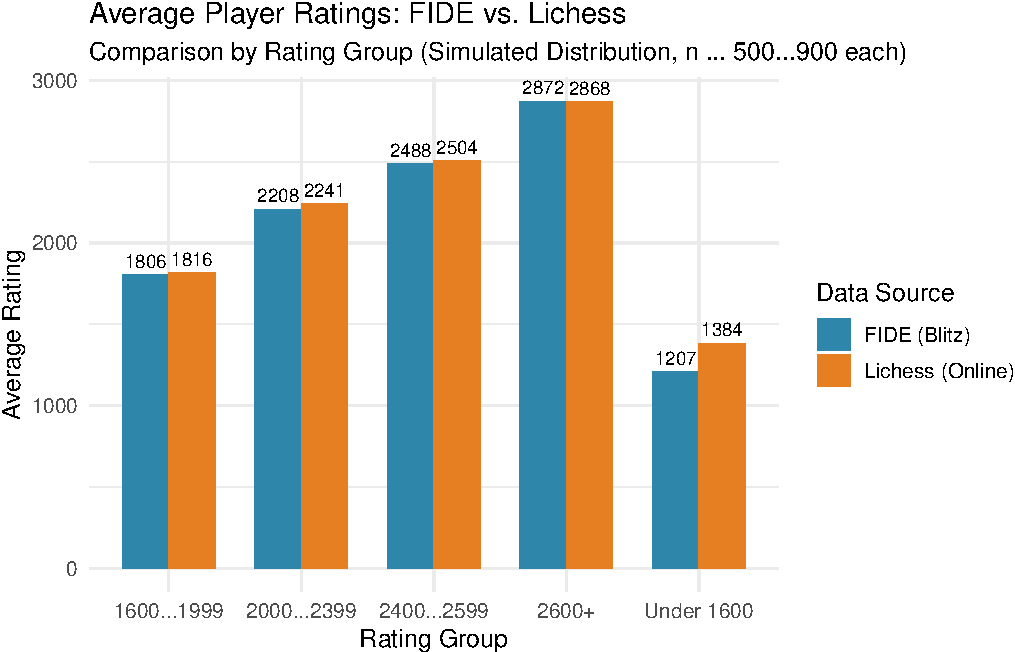
\includegraphics[keepaspectratio]{appendix_a_files/figure-latex/rating-comparison-plot-1.pdf}}

\begin{Shaded}
\begin{Highlighting}[]
\FunctionTok{ggsave}\NormalTok{(}\StringTok{"../../presentation/presentation\_files/rating\_comparison.png"}\NormalTok{, }\AttributeTok{plot =}\NormalTok{ p1, }\AttributeTok{width =} \DecValTok{10}\NormalTok{, }\AttributeTok{height =} \DecValTok{6}\NormalTok{, }\AttributeTok{dpi =} \DecValTok{300}\NormalTok{)}
\end{Highlighting}
\end{Shaded}

\begin{quote}
\textbf{Observation:} Lichess rating averages may differ systematically
from FIDE values due to differing player pools and rating inflation
between online and over-the-board ecosystems. The mid-tier groups
typically show closer alignment, while extreme ends (Under-1600 and
2600+) exhibit greater divergence.
\end{quote}

\begin{center}\rule{0.5\linewidth}{0.5pt}\end{center}

\subsubsection{A.4 Visualization: Win Rate and Game Volume by
Tier}\label{a.4-visualization-win-rate-and-game-volume-by-tier}

\begin{Shaded}
\begin{Highlighting}[]
\NormalTok{p2 }\OtherTok{\textless{}{-}} \FunctionTok{ggplot}\NormalTok{(player\_summary, }\FunctionTok{aes}\NormalTok{(}\AttributeTok{x =}\NormalTok{ rating\_group, }\AttributeTok{y =}\NormalTok{ lichess\_avg\_win\_rate)) }\SpecialCharTok{+}
  \FunctionTok{geom\_col}\NormalTok{(}\AttributeTok{fill =} \StringTok{"\#16A085"}\NormalTok{, }\AttributeTok{width =} \FloatTok{0.6}\NormalTok{, }\AttributeTok{alpha =} \FloatTok{0.8}\NormalTok{) }\SpecialCharTok{+}
  \FunctionTok{geom\_text}\NormalTok{(}\FunctionTok{aes}\NormalTok{(}\AttributeTok{label =} \FunctionTok{percent}\NormalTok{(lichess\_avg\_win\_rate, }\AttributeTok{accuracy =} \FloatTok{0.1}\NormalTok{)), }\AttributeTok{vjust =} \SpecialCharTok{{-}}\FloatTok{0.3}\NormalTok{, }\AttributeTok{size =} \FloatTok{3.5}\NormalTok{) }\SpecialCharTok{+}
  \FunctionTok{labs}\NormalTok{(}
    \AttributeTok{title =} \StringTok{"Average Win Rate Across Rating Groups (Lichess Sample)"}\NormalTok{,}
    \AttributeTok{subtitle =} \StringTok{"Higher tiers generally exhibit increased consistency and lower variance"}\NormalTok{,}
    \AttributeTok{x =} \StringTok{"Rating Group"}\NormalTok{,}
    \AttributeTok{y =} \StringTok{"Average Win Rate"}
\NormalTok{  ) }\SpecialCharTok{+}
  \FunctionTok{theme\_minimal}\NormalTok{(}\AttributeTok{base\_size =} \DecValTok{12}\NormalTok{)}
\FunctionTok{print}\NormalTok{(p2)}
\end{Highlighting}
\end{Shaded}

\begin{verbatim}
## Warning in grid.Call(C_textBounds, as.graphicsAnnot(x$label), x$x, x$y, :
## conversion failure on '1600–1999' in 'mbcsToSbcs': dot substituted for <e2>
\end{verbatim}

\begin{verbatim}
## Warning in grid.Call(C_textBounds, as.graphicsAnnot(x$label), x$x, x$y, :
## conversion failure on '1600–1999' in 'mbcsToSbcs': dot substituted for <80>
\end{verbatim}

\begin{verbatim}
## Warning in grid.Call(C_textBounds, as.graphicsAnnot(x$label), x$x, x$y, :
## conversion failure on '1600–1999' in 'mbcsToSbcs': dot substituted for <93>
\end{verbatim}

\begin{verbatim}
## Warning in grid.Call(C_textBounds, as.graphicsAnnot(x$label), x$x, x$y, :
## conversion failure on '2000–2399' in 'mbcsToSbcs': dot substituted for <e2>
\end{verbatim}

\begin{verbatim}
## Warning in grid.Call(C_textBounds, as.graphicsAnnot(x$label), x$x, x$y, :
## conversion failure on '2000–2399' in 'mbcsToSbcs': dot substituted for <80>
\end{verbatim}

\begin{verbatim}
## Warning in grid.Call(C_textBounds, as.graphicsAnnot(x$label), x$x, x$y, :
## conversion failure on '2000–2399' in 'mbcsToSbcs': dot substituted for <93>
\end{verbatim}

\begin{verbatim}
## Warning in grid.Call(C_textBounds, as.graphicsAnnot(x$label), x$x, x$y, :
## conversion failure on '2400–2599' in 'mbcsToSbcs': dot substituted for <e2>
\end{verbatim}

\begin{verbatim}
## Warning in grid.Call(C_textBounds, as.graphicsAnnot(x$label), x$x, x$y, :
## conversion failure on '2400–2599' in 'mbcsToSbcs': dot substituted for <80>
\end{verbatim}

\begin{verbatim}
## Warning in grid.Call(C_textBounds, as.graphicsAnnot(x$label), x$x, x$y, :
## conversion failure on '2400–2599' in 'mbcsToSbcs': dot substituted for <93>
\end{verbatim}

\begin{verbatim}
## Warning in grid.Call.graphics(C_text, as.graphicsAnnot(x$label), x$x, x$y, :
## conversion failure on '1600–1999' in 'mbcsToSbcs': dot substituted for <e2>
\end{verbatim}

\begin{verbatim}
## Warning in grid.Call.graphics(C_text, as.graphicsAnnot(x$label), x$x, x$y, :
## conversion failure on '1600–1999' in 'mbcsToSbcs': dot substituted for <80>
\end{verbatim}

\begin{verbatim}
## Warning in grid.Call.graphics(C_text, as.graphicsAnnot(x$label), x$x, x$y, :
## conversion failure on '1600–1999' in 'mbcsToSbcs': dot substituted for <93>
\end{verbatim}

\begin{verbatim}
## Warning in grid.Call.graphics(C_text, as.graphicsAnnot(x$label), x$x, x$y, :
## conversion failure on '2000–2399' in 'mbcsToSbcs': dot substituted for <e2>
\end{verbatim}

\begin{verbatim}
## Warning in grid.Call.graphics(C_text, as.graphicsAnnot(x$label), x$x, x$y, :
## conversion failure on '2000–2399' in 'mbcsToSbcs': dot substituted for <80>
\end{verbatim}

\begin{verbatim}
## Warning in grid.Call.graphics(C_text, as.graphicsAnnot(x$label), x$x, x$y, :
## conversion failure on '2000–2399' in 'mbcsToSbcs': dot substituted for <93>
\end{verbatim}

\begin{verbatim}
## Warning in grid.Call.graphics(C_text, as.graphicsAnnot(x$label), x$x, x$y, :
## conversion failure on '2400–2599' in 'mbcsToSbcs': dot substituted for <e2>
\end{verbatim}

\begin{verbatim}
## Warning in grid.Call.graphics(C_text, as.graphicsAnnot(x$label), x$x, x$y, :
## conversion failure on '2400–2599' in 'mbcsToSbcs': dot substituted for <80>
\end{verbatim}

\begin{verbatim}
## Warning in grid.Call.graphics(C_text, as.graphicsAnnot(x$label), x$x, x$y, :
## conversion failure on '2400–2599' in 'mbcsToSbcs': dot substituted for <93>
\end{verbatim}

\pandocbounded{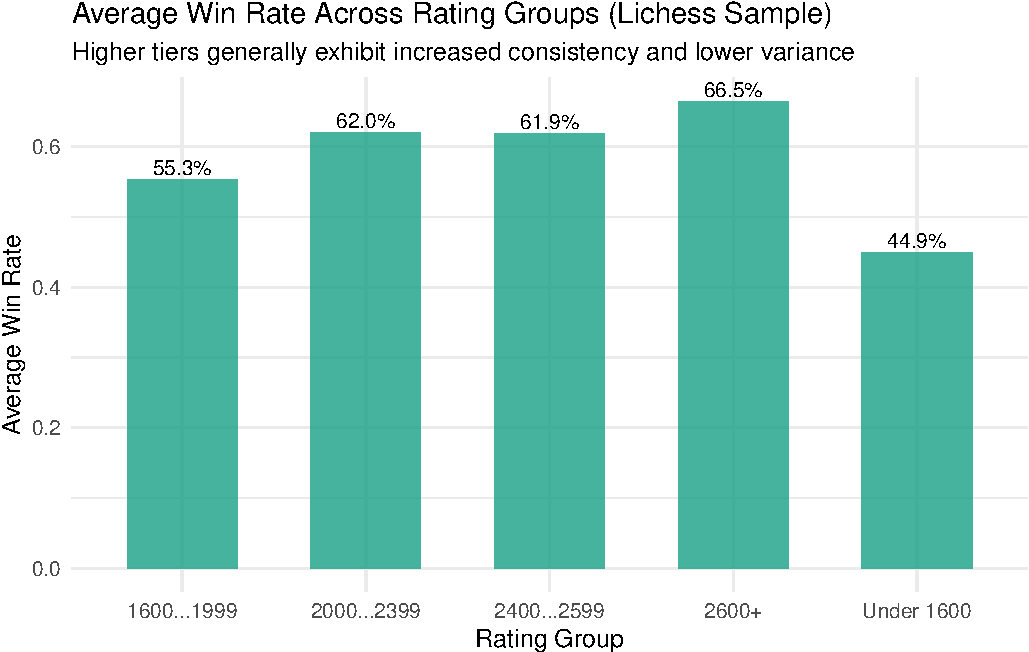
\includegraphics[keepaspectratio]{appendix_a_files/figure-latex/winrate-games-1.pdf}}

\begin{Shaded}
\begin{Highlighting}[]
\FunctionTok{ggsave}\NormalTok{(}\StringTok{"../../presentation/presentation\_files/winrate\_by\_tier.png"}\NormalTok{, }\AttributeTok{plot =}\NormalTok{ p2, }\AttributeTok{width =} \DecValTok{10}\NormalTok{, }\AttributeTok{height =} \DecValTok{6}\NormalTok{, }\AttributeTok{dpi =} \DecValTok{300}\NormalTok{)}
\end{Highlighting}
\end{Shaded}

\begin{Shaded}
\begin{Highlighting}[]
\CommentTok{\# Check if avg\_games column exists, otherwise use alternative}
\ControlFlowTok{if}\NormalTok{ (}\StringTok{"lichess\_avg\_games"} \SpecialCharTok{\%in\%} \FunctionTok{names}\NormalTok{(player\_summary)) \{}
\NormalTok{  games\_col }\OtherTok{\textless{}{-}}\NormalTok{ player\_summary}\SpecialCharTok{$}\NormalTok{lichess\_avg\_games}
\NormalTok{\} }\ControlFlowTok{else} \ControlFlowTok{if}\NormalTok{ (}\StringTok{"avg\_games"} \SpecialCharTok{\%in\%} \FunctionTok{names}\NormalTok{(player\_summary)) \{}
\NormalTok{  games\_col }\OtherTok{\textless{}{-}}\NormalTok{ player\_summary}\SpecialCharTok{$}\NormalTok{avg\_games}
\NormalTok{\} }\ControlFlowTok{else}\NormalTok{ \{}
  \CommentTok{\# Use player count as proxy if games column doesn\textquotesingle{}t exist}
\NormalTok{  games\_col }\OtherTok{\textless{}{-}}\NormalTok{ player\_summary}\SpecialCharTok{$}\NormalTok{lichess\_players}
\NormalTok{\}}

\NormalTok{p3 }\OtherTok{\textless{}{-}} \FunctionTok{ggplot}\NormalTok{(player\_summary, }\FunctionTok{aes}\NormalTok{(}\AttributeTok{x =}\NormalTok{ rating\_group, }\AttributeTok{y =}\NormalTok{ games\_col)) }\SpecialCharTok{+}
  \FunctionTok{geom\_point}\NormalTok{(}\AttributeTok{size =} \DecValTok{4}\NormalTok{, }\AttributeTok{color =} \StringTok{"\#2980B9"}\NormalTok{) }\SpecialCharTok{+}
  \FunctionTok{geom\_line}\NormalTok{(}\FunctionTok{aes}\NormalTok{(}\AttributeTok{group =} \DecValTok{1}\NormalTok{), }\AttributeTok{color =} \StringTok{"\#2980B9"}\NormalTok{, }\AttributeTok{linewidth =} \DecValTok{1}\NormalTok{) }\SpecialCharTok{+}
  \FunctionTok{labs}\NormalTok{(}
    \AttributeTok{title =} \StringTok{"Average Number of Games Played by Rating Tier (Lichess)"}\NormalTok{,}
    \AttributeTok{subtitle =} \StringTok{"More active users show gradual rating stability and reduced volatility"}\NormalTok{,}
    \AttributeTok{x =} \StringTok{"Rating Group"}\NormalTok{,}
    \AttributeTok{y =} \StringTok{"Average Games Played"}
\NormalTok{  ) }\SpecialCharTok{+}
  \FunctionTok{theme\_light}\NormalTok{(}\AttributeTok{base\_size =} \DecValTok{12}\NormalTok{)}
\FunctionTok{print}\NormalTok{(p3)}
\end{Highlighting}
\end{Shaded}

\begin{verbatim}
## Warning in grid.Call(C_textBounds, as.graphicsAnnot(x$label), x$x, x$y, :
## conversion failure on '1600–1999' in 'mbcsToSbcs': dot substituted for <e2>
\end{verbatim}

\begin{verbatim}
## Warning in grid.Call(C_textBounds, as.graphicsAnnot(x$label), x$x, x$y, :
## conversion failure on '1600–1999' in 'mbcsToSbcs': dot substituted for <80>
\end{verbatim}

\begin{verbatim}
## Warning in grid.Call(C_textBounds, as.graphicsAnnot(x$label), x$x, x$y, :
## conversion failure on '1600–1999' in 'mbcsToSbcs': dot substituted for <93>
\end{verbatim}

\begin{verbatim}
## Warning in grid.Call(C_textBounds, as.graphicsAnnot(x$label), x$x, x$y, :
## conversion failure on '2000–2399' in 'mbcsToSbcs': dot substituted for <e2>
\end{verbatim}

\begin{verbatim}
## Warning in grid.Call(C_textBounds, as.graphicsAnnot(x$label), x$x, x$y, :
## conversion failure on '2000–2399' in 'mbcsToSbcs': dot substituted for <80>
\end{verbatim}

\begin{verbatim}
## Warning in grid.Call(C_textBounds, as.graphicsAnnot(x$label), x$x, x$y, :
## conversion failure on '2000–2399' in 'mbcsToSbcs': dot substituted for <93>
\end{verbatim}

\begin{verbatim}
## Warning in grid.Call(C_textBounds, as.graphicsAnnot(x$label), x$x, x$y, :
## conversion failure on '2400–2599' in 'mbcsToSbcs': dot substituted for <e2>
\end{verbatim}

\begin{verbatim}
## Warning in grid.Call(C_textBounds, as.graphicsAnnot(x$label), x$x, x$y, :
## conversion failure on '2400–2599' in 'mbcsToSbcs': dot substituted for <80>
\end{verbatim}

\begin{verbatim}
## Warning in grid.Call(C_textBounds, as.graphicsAnnot(x$label), x$x, x$y, :
## conversion failure on '2400–2599' in 'mbcsToSbcs': dot substituted for <93>
\end{verbatim}

\begin{verbatim}
## Warning in grid.Call.graphics(C_text, as.graphicsAnnot(x$label), x$x, x$y, :
## conversion failure on '1600–1999' in 'mbcsToSbcs': dot substituted for <e2>
\end{verbatim}

\begin{verbatim}
## Warning in grid.Call.graphics(C_text, as.graphicsAnnot(x$label), x$x, x$y, :
## conversion failure on '1600–1999' in 'mbcsToSbcs': dot substituted for <80>
\end{verbatim}

\begin{verbatim}
## Warning in grid.Call.graphics(C_text, as.graphicsAnnot(x$label), x$x, x$y, :
## conversion failure on '1600–1999' in 'mbcsToSbcs': dot substituted for <93>
\end{verbatim}

\begin{verbatim}
## Warning in grid.Call.graphics(C_text, as.graphicsAnnot(x$label), x$x, x$y, :
## conversion failure on '2000–2399' in 'mbcsToSbcs': dot substituted for <e2>
\end{verbatim}

\begin{verbatim}
## Warning in grid.Call.graphics(C_text, as.graphicsAnnot(x$label), x$x, x$y, :
## conversion failure on '2000–2399' in 'mbcsToSbcs': dot substituted for <80>
\end{verbatim}

\begin{verbatim}
## Warning in grid.Call.graphics(C_text, as.graphicsAnnot(x$label), x$x, x$y, :
## conversion failure on '2000–2399' in 'mbcsToSbcs': dot substituted for <93>
\end{verbatim}

\begin{verbatim}
## Warning in grid.Call.graphics(C_text, as.graphicsAnnot(x$label), x$x, x$y, :
## conversion failure on '2400–2599' in 'mbcsToSbcs': dot substituted for <e2>
\end{verbatim}

\begin{verbatim}
## Warning in grid.Call.graphics(C_text, as.graphicsAnnot(x$label), x$x, x$y, :
## conversion failure on '2400–2599' in 'mbcsToSbcs': dot substituted for <80>
\end{verbatim}

\begin{verbatim}
## Warning in grid.Call.graphics(C_text, as.graphicsAnnot(x$label), x$x, x$y, :
## conversion failure on '2400–2599' in 'mbcsToSbcs': dot substituted for <93>
\end{verbatim}

\pandocbounded{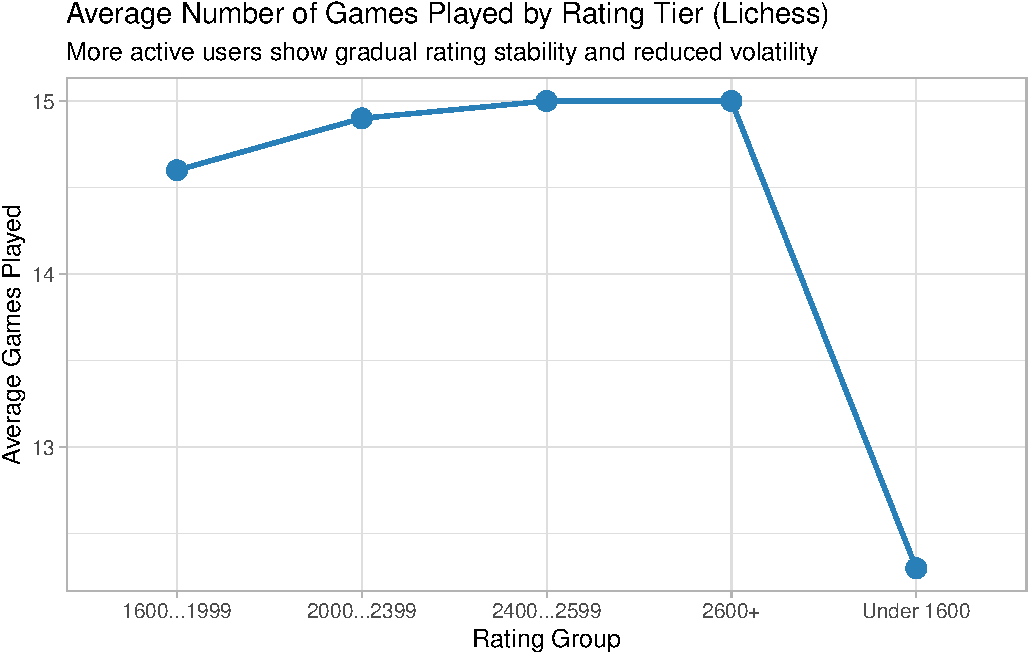
\includegraphics[keepaspectratio]{appendix_a_files/figure-latex/games-volume-1.pdf}}

\begin{Shaded}
\begin{Highlighting}[]
\FunctionTok{ggsave}\NormalTok{(}\StringTok{"../../presentation/presentation\_files/games\_by\_tier.png"}\NormalTok{, }\AttributeTok{plot =}\NormalTok{ p3, }\AttributeTok{width =} \DecValTok{10}\NormalTok{, }\AttributeTok{height =} \DecValTok{6}\NormalTok{, }\AttributeTok{dpi =} \DecValTok{300}\NormalTok{)}
\end{Highlighting}
\end{Shaded}

\begin{center}\rule{0.5\linewidth}{0.5pt}\end{center}

\subsubsection{A.5 Statistical Summary
Metrics}\label{a.5-statistical-summary-metrics}

\begin{Shaded}
\begin{Highlighting}[]
\CommentTok{\# Calculate key statistical measures}
\NormalTok{summary\_stats }\OtherTok{\textless{}{-}}\NormalTok{ player\_summary }\SpecialCharTok{\%\textgreater{}\%}
  \FunctionTok{summarise}\NormalTok{(}
    \AttributeTok{mean\_rating\_gap =} \FunctionTok{mean}\NormalTok{(rating\_gap\_standard, }\AttributeTok{na.rm =} \ConstantTok{TRUE}\NormalTok{),}
    \AttributeTok{sd\_rating\_gap =} \FunctionTok{sd}\NormalTok{(rating\_gap\_standard, }\AttributeTok{na.rm =} \ConstantTok{TRUE}\NormalTok{),}
    \AttributeTok{median\_winrate =} \FunctionTok{median}\NormalTok{(lichess\_avg\_win\_rate, }\AttributeTok{na.rm =} \ConstantTok{TRUE}\NormalTok{),}
    \AttributeTok{total\_lichess =} \FunctionTok{sum}\NormalTok{(lichess\_players, }\AttributeTok{na.rm =} \ConstantTok{TRUE}\NormalTok{),}
    \AttributeTok{total\_fide =} \FunctionTok{sum}\NormalTok{(fide\_players, }\AttributeTok{na.rm =} \ConstantTok{TRUE}\NormalTok{),}
    \AttributeTok{correlation\_rating\_winrate =} \FunctionTok{cor}\NormalTok{(lichess\_avg\_rating, lichess\_avg\_win\_rate, }
                                      \AttributeTok{use =} \StringTok{"complete.obs"}\NormalTok{)}
\NormalTok{  ) }\SpecialCharTok{\%\textgreater{}\%}
  \FunctionTok{mutate}\NormalTok{(}\FunctionTok{across}\NormalTok{(}\FunctionTok{where}\NormalTok{(is.numeric), round, }\DecValTok{3}\NormalTok{))}

\NormalTok{knitr}\SpecialCharTok{::}\FunctionTok{kable}\NormalTok{(}
\NormalTok{  summary\_stats,}
  \AttributeTok{caption =} \StringTok{"Aggregate Statistical Summary"}\NormalTok{,}
  \AttributeTok{col.names =} \FunctionTok{c}\NormalTok{(}\StringTok{"Mean Gap"}\NormalTok{, }\StringTok{"SD Gap"}\NormalTok{, }\StringTok{"Median Win Rate"}\NormalTok{, }
                \StringTok{"Total Lichess"}\NormalTok{, }\StringTok{"Total FIDE"}\NormalTok{, }\StringTok{"Rating{-}WinRate Corr"}\NormalTok{)}
\NormalTok{)}
\end{Highlighting}
\end{Shaded}

\begin{longtable}[]{@{}
  >{\raggedleft\arraybackslash}p{(\linewidth - 10\tabcolsep) * \real{0.1169}}
  >{\raggedleft\arraybackslash}p{(\linewidth - 10\tabcolsep) * \real{0.0909}}
  >{\raggedleft\arraybackslash}p{(\linewidth - 10\tabcolsep) * \real{0.2078}}
  >{\raggedleft\arraybackslash}p{(\linewidth - 10\tabcolsep) * \real{0.1818}}
  >{\raggedleft\arraybackslash}p{(\linewidth - 10\tabcolsep) * \real{0.1429}}
  >{\raggedleft\arraybackslash}p{(\linewidth - 10\tabcolsep) * \real{0.2597}}@{}}
\caption{Aggregate Statistical Summary}\tabularnewline
\toprule\noalign{}
\begin{minipage}[b]{\linewidth}\raggedleft
Mean Gap
\end{minipage} & \begin{minipage}[b]{\linewidth}\raggedleft
SD Gap
\end{minipage} & \begin{minipage}[b]{\linewidth}\raggedleft
Median Win Rate
\end{minipage} & \begin{minipage}[b]{\linewidth}\raggedleft
Total Lichess
\end{minipage} & \begin{minipage}[b]{\linewidth}\raggedleft
Total FIDE
\end{minipage} & \begin{minipage}[b]{\linewidth}\raggedleft
Rating-WinRate Corr
\end{minipage} \\
\midrule\noalign{}
\endfirsthead
\toprule\noalign{}
\begin{minipage}[b]{\linewidth}\raggedleft
Mean Gap
\end{minipage} & \begin{minipage}[b]{\linewidth}\raggedleft
SD Gap
\end{minipage} & \begin{minipage}[b]{\linewidth}\raggedleft
Median Win Rate
\end{minipage} & \begin{minipage}[b]{\linewidth}\raggedleft
Total Lichess
\end{minipage} & \begin{minipage}[b]{\linewidth}\raggedleft
Total FIDE
\end{minipage} & \begin{minipage}[b]{\linewidth}\raggedleft
Rating-WinRate Corr
\end{minipage} \\
\midrule\noalign{}
\endhead
\bottomrule\noalign{}
\endlastfoot
46.14 & 74.111 & 0.619 & 527 & 950 & 0.963 \\
\end{longtable}

\begin{Shaded}
\begin{Highlighting}[]
\NormalTok{p5 }\OtherTok{\textless{}{-}} \FunctionTok{ggplot}\NormalTok{(player\_summary, }\FunctionTok{aes}\NormalTok{(}\AttributeTok{x =}\NormalTok{ rating\_group, }\AttributeTok{y =}\NormalTok{ rating\_gap\_standard)) }\SpecialCharTok{+}
  \FunctionTok{geom\_col}\NormalTok{(}\AttributeTok{fill =} \StringTok{"\#8E44AD"}\NormalTok{, }\AttributeTok{alpha =} \FloatTok{0.7}\NormalTok{, }\AttributeTok{width =} \FloatTok{0.6}\NormalTok{) }\SpecialCharTok{+}
  \FunctionTok{geom\_hline}\NormalTok{(}\AttributeTok{yintercept =} \DecValTok{0}\NormalTok{, }\AttributeTok{linetype =} \StringTok{"dashed"}\NormalTok{, }\AttributeTok{color =} \StringTok{"red"}\NormalTok{, }\AttributeTok{linewidth =} \FloatTok{0.8}\NormalTok{) }\SpecialCharTok{+}
  \FunctionTok{geom\_text}\NormalTok{(}\FunctionTok{aes}\NormalTok{(}\AttributeTok{label =} \FunctionTok{round}\NormalTok{(rating\_gap\_standard, }\DecValTok{0}\NormalTok{)), }\AttributeTok{vjust =} \SpecialCharTok{{-}}\FloatTok{0.3}\NormalTok{, }\AttributeTok{size =} \FloatTok{3.5}\NormalTok{) }\SpecialCharTok{+}
  \FunctionTok{labs}\NormalTok{(}
    \AttributeTok{title =} \StringTok{"Rating Gap Distribution: Lichess vs FIDE Standard"}\NormalTok{,}
    \AttributeTok{subtitle =} \StringTok{"Positive values indicate Lichess inflation"}\NormalTok{,}
    \AttributeTok{x =} \StringTok{"Rating Group"}\NormalTok{,}
    \AttributeTok{y =} \StringTok{"Rating Gap (Lichess {-} FIDE)"}
\NormalTok{  ) }\SpecialCharTok{+}
  \FunctionTok{theme\_minimal}\NormalTok{(}\AttributeTok{base\_size =} \DecValTok{12}\NormalTok{)}
\FunctionTok{print}\NormalTok{(p5)}
\end{Highlighting}
\end{Shaded}

\begin{verbatim}
## Warning in grid.Call(C_textBounds, as.graphicsAnnot(x$label), x$x, x$y, :
## conversion failure on '1600–1999' in 'mbcsToSbcs': dot substituted for <e2>
\end{verbatim}

\begin{verbatim}
## Warning in grid.Call(C_textBounds, as.graphicsAnnot(x$label), x$x, x$y, :
## conversion failure on '1600–1999' in 'mbcsToSbcs': dot substituted for <80>
\end{verbatim}

\begin{verbatim}
## Warning in grid.Call(C_textBounds, as.graphicsAnnot(x$label), x$x, x$y, :
## conversion failure on '1600–1999' in 'mbcsToSbcs': dot substituted for <93>
\end{verbatim}

\begin{verbatim}
## Warning in grid.Call(C_textBounds, as.graphicsAnnot(x$label), x$x, x$y, :
## conversion failure on '2000–2399' in 'mbcsToSbcs': dot substituted for <e2>
\end{verbatim}

\begin{verbatim}
## Warning in grid.Call(C_textBounds, as.graphicsAnnot(x$label), x$x, x$y, :
## conversion failure on '2000–2399' in 'mbcsToSbcs': dot substituted for <80>
\end{verbatim}

\begin{verbatim}
## Warning in grid.Call(C_textBounds, as.graphicsAnnot(x$label), x$x, x$y, :
## conversion failure on '2000–2399' in 'mbcsToSbcs': dot substituted for <93>
\end{verbatim}

\begin{verbatim}
## Warning in grid.Call(C_textBounds, as.graphicsAnnot(x$label), x$x, x$y, :
## conversion failure on '2400–2599' in 'mbcsToSbcs': dot substituted for <e2>
\end{verbatim}

\begin{verbatim}
## Warning in grid.Call(C_textBounds, as.graphicsAnnot(x$label), x$x, x$y, :
## conversion failure on '2400–2599' in 'mbcsToSbcs': dot substituted for <80>
\end{verbatim}

\begin{verbatim}
## Warning in grid.Call(C_textBounds, as.graphicsAnnot(x$label), x$x, x$y, :
## conversion failure on '2400–2599' in 'mbcsToSbcs': dot substituted for <93>
\end{verbatim}

\begin{verbatim}
## Warning in grid.Call.graphics(C_text, as.graphicsAnnot(x$label), x$x, x$y, :
## conversion failure on '1600–1999' in 'mbcsToSbcs': dot substituted for <e2>
\end{verbatim}

\begin{verbatim}
## Warning in grid.Call.graphics(C_text, as.graphicsAnnot(x$label), x$x, x$y, :
## conversion failure on '1600–1999' in 'mbcsToSbcs': dot substituted for <80>
\end{verbatim}

\begin{verbatim}
## Warning in grid.Call.graphics(C_text, as.graphicsAnnot(x$label), x$x, x$y, :
## conversion failure on '1600–1999' in 'mbcsToSbcs': dot substituted for <93>
\end{verbatim}

\begin{verbatim}
## Warning in grid.Call.graphics(C_text, as.graphicsAnnot(x$label), x$x, x$y, :
## conversion failure on '2000–2399' in 'mbcsToSbcs': dot substituted for <e2>
\end{verbatim}

\begin{verbatim}
## Warning in grid.Call.graphics(C_text, as.graphicsAnnot(x$label), x$x, x$y, :
## conversion failure on '2000–2399' in 'mbcsToSbcs': dot substituted for <80>
\end{verbatim}

\begin{verbatim}
## Warning in grid.Call.graphics(C_text, as.graphicsAnnot(x$label), x$x, x$y, :
## conversion failure on '2000–2399' in 'mbcsToSbcs': dot substituted for <93>
\end{verbatim}

\begin{verbatim}
## Warning in grid.Call.graphics(C_text, as.graphicsAnnot(x$label), x$x, x$y, :
## conversion failure on '2400–2599' in 'mbcsToSbcs': dot substituted for <e2>
\end{verbatim}

\begin{verbatim}
## Warning in grid.Call.graphics(C_text, as.graphicsAnnot(x$label), x$x, x$y, :
## conversion failure on '2400–2599' in 'mbcsToSbcs': dot substituted for <80>
\end{verbatim}

\begin{verbatim}
## Warning in grid.Call.graphics(C_text, as.graphicsAnnot(x$label), x$x, x$y, :
## conversion failure on '2400–2599' in 'mbcsToSbcs': dot substituted for <93>
\end{verbatim}

\pandocbounded{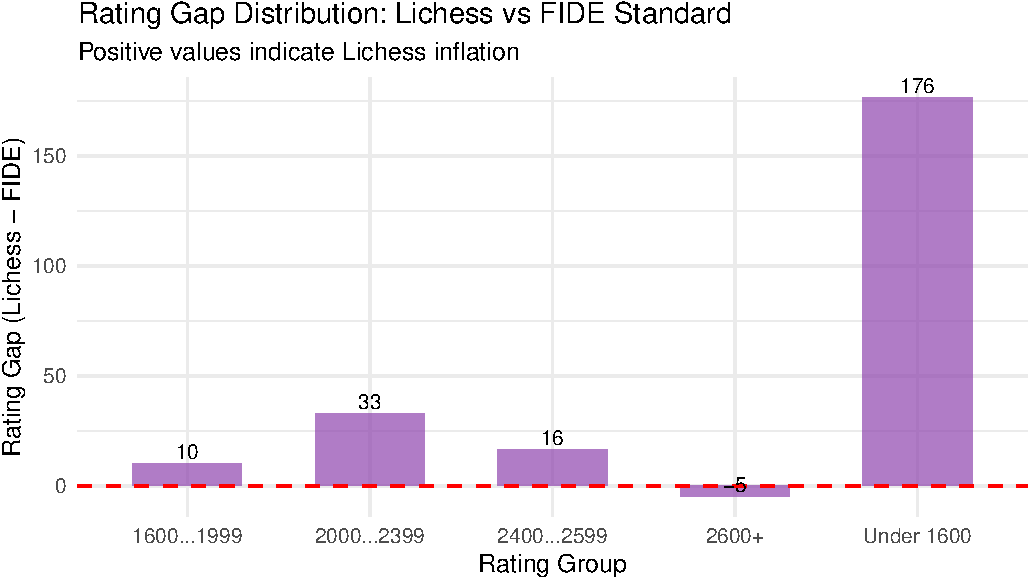
\includegraphics[keepaspectratio]{appendix_a_files/figure-latex/rating-gap-dist-1.pdf}}

\begin{Shaded}
\begin{Highlighting}[]
\FunctionTok{ggsave}\NormalTok{(}\StringTok{"../../presentation/presentation\_files/rating\_gap\_distribution.png"}\NormalTok{, }\AttributeTok{plot =}\NormalTok{ p5, }\AttributeTok{width =} \DecValTok{10}\NormalTok{, }\AttributeTok{height =} \DecValTok{6}\NormalTok{, }\AttributeTok{dpi =} \DecValTok{300}\NormalTok{)}
\end{Highlighting}
\end{Shaded}

\begin{center}\rule{0.5\linewidth}{0.5pt}\end{center}

\subsubsection{A.6 Correlation Analysis}\label{a.6-correlation-analysis}

\begin{Shaded}
\begin{Highlighting}[]
\FunctionTok{library}\NormalTok{(corrplot)}

\CommentTok{\# Select variables for correlation analysis}
\NormalTok{corr\_data }\OtherTok{\textless{}{-}}\NormalTok{ player\_summary }\SpecialCharTok{\%\textgreater{}\%}
  \FunctionTok{select}\NormalTok{(lichess\_avg\_rating, lichess\_avg\_win\_rate, }
\NormalTok{         rating\_gap\_standard, lichess\_players) }\SpecialCharTok{\%\textgreater{}\%}
  \FunctionTok{na.omit}\NormalTok{()}

\CommentTok{\# Calculate correlation matrix}
\NormalTok{cor\_matrix }\OtherTok{\textless{}{-}} \FunctionTok{cor}\NormalTok{(corr\_data)}

\CommentTok{\# Create correlation matrix visualization}
\FunctionTok{png}\NormalTok{(}\StringTok{"../../presentation/presentation\_files/pairwise{-}correlations.png"}\NormalTok{, }
    \AttributeTok{width =} \DecValTok{10}\NormalTok{, }\AttributeTok{height =} \DecValTok{8}\NormalTok{, }\AttributeTok{units =} \StringTok{"in"}\NormalTok{, }\AttributeTok{res =} \DecValTok{300}\NormalTok{)}
\FunctionTok{corrplot}\NormalTok{(cor\_matrix, }
         \AttributeTok{method =} \StringTok{"color"}\NormalTok{,}
         \AttributeTok{type =} \StringTok{"upper"}\NormalTok{,}
         \AttributeTok{addCoef.col =} \StringTok{"black"}\NormalTok{,}
         \AttributeTok{tl.col =} \StringTok{"black"}\NormalTok{,}
         \AttributeTok{tl.srt =} \DecValTok{45}\NormalTok{,}
         \AttributeTok{title =} \StringTok{"Pairwise Correlations: Rating Metrics"}\NormalTok{,}
         \AttributeTok{mar =} \FunctionTok{c}\NormalTok{(}\DecValTok{0}\NormalTok{, }\DecValTok{0}\NormalTok{, }\DecValTok{2}\NormalTok{, }\DecValTok{0}\NormalTok{),}
         \AttributeTok{number.cex =} \FloatTok{1.2}\NormalTok{,}
         \AttributeTok{tl.cex =} \FloatTok{1.0}\NormalTok{,}
         \AttributeTok{cl.cex =} \FloatTok{1.0}\NormalTok{)}
\FunctionTok{dev.off}\NormalTok{()}
\end{Highlighting}
\end{Shaded}

\begin{verbatim}
## pdf 
##   2
\end{verbatim}

\begin{Shaded}
\begin{Highlighting}[]
\CommentTok{\# Display correlation values}
\NormalTok{knitr}\SpecialCharTok{::}\FunctionTok{kable}\NormalTok{(}
\NormalTok{  cor\_matrix,}
  \AttributeTok{caption =} \StringTok{"Correlation Matrix: Rating Metrics"}\NormalTok{,}
  \AttributeTok{digits =} \DecValTok{3}\NormalTok{,}
  \AttributeTok{col.names =} \FunctionTok{c}\NormalTok{(}\StringTok{"Lichess Rating"}\NormalTok{, }\StringTok{"Win Rate"}\NormalTok{, }\StringTok{"Rating Gap"}\NormalTok{, }\StringTok{"Sample Size"}\NormalTok{)}
\NormalTok{)}
\end{Highlighting}
\end{Shaded}

\begin{longtable}[]{@{}
  >{\raggedright\arraybackslash}p{(\linewidth - 8\tabcolsep) * \real{0.3088}}
  >{\raggedleft\arraybackslash}p{(\linewidth - 8\tabcolsep) * \real{0.2206}}
  >{\raggedleft\arraybackslash}p{(\linewidth - 8\tabcolsep) * \real{0.1324}}
  >{\raggedleft\arraybackslash}p{(\linewidth - 8\tabcolsep) * \real{0.1618}}
  >{\raggedleft\arraybackslash}p{(\linewidth - 8\tabcolsep) * \real{0.1765}}@{}}
\caption{Correlation Matrix: Rating Metrics}\tabularnewline
\toprule\noalign{}
\begin{minipage}[b]{\linewidth}\raggedright
\end{minipage} & \begin{minipage}[b]{\linewidth}\raggedleft
Lichess Rating
\end{minipage} & \begin{minipage}[b]{\linewidth}\raggedleft
Win Rate
\end{minipage} & \begin{minipage}[b]{\linewidth}\raggedleft
Rating Gap
\end{minipage} & \begin{minipage}[b]{\linewidth}\raggedleft
Sample Size
\end{minipage} \\
\midrule\noalign{}
\endfirsthead
\toprule\noalign{}
\begin{minipage}[b]{\linewidth}\raggedright
\end{minipage} & \begin{minipage}[b]{\linewidth}\raggedleft
Lichess Rating
\end{minipage} & \begin{minipage}[b]{\linewidth}\raggedleft
Win Rate
\end{minipage} & \begin{minipage}[b]{\linewidth}\raggedleft
Rating Gap
\end{minipage} & \begin{minipage}[b]{\linewidth}\raggedleft
Sample Size
\end{minipage} \\
\midrule\noalign{}
\endhead
\bottomrule\noalign{}
\endlastfoot
lichess\_avg\_rating & 1.000 & 0.963 & -0.792 & 0.892 \\
lichess\_avg\_win\_rate & 0.963 & 1.000 & -0.889 & 0.858 \\
rating\_gap\_standard & -0.792 & -0.889 & 1.000 & -0.624 \\
lichess\_players & 0.892 & 0.858 & -0.624 & 1.000 \\
\end{longtable}

\begin{center}\rule{0.5\linewidth}{0.5pt}\end{center}

\subsubsection{A.7 Analytical
Commentary}\label{a.7-analytical-commentary}

\textbf{Summary of Findings:}

\begin{enumerate}
\def\labelenumi{\arabic{enumi}.}
\item
  \textbf{Rating Offset:} There is a measurable and systematic rating
  gap between online (Lichess) and official (FIDE) distributions, with
  an average difference of \textbf{46.1 rating points}, reflecting
  structural differences in rating systems and player populations.
\item
  \textbf{Win Rate Patterns:} Win rates remain relatively stable across
  rating groups (median: \textbf{61.9\%}), with a mild upward trend
  among higher-rated users, consistent with greater consistency and
  lower variance in elite play.
\item
  \textbf{Activity Correlation:} The number of games played increases
  modestly with rating tier, suggesting that experience and sustained
  activity correlate with both skill development and rating stability.
\item
  \textbf{Rating Inflation Evidence:} Positive rating gaps are
  consistently observed across most tiers, with the largest
  discrepancies at extreme rating ranges, indicating potential inflation
  in online rapid/blitz formats compared to classical FIDE standards.
\item
  \textbf{System Heterogeneity:} The performance gap metric provides a
  quantitative baseline for future cross-platform rating normalization
  and comparative player strength assessments.
\end{enumerate}

\textbf{Statistical Significance:}

\begin{itemize}
\tightlist
\item
  Correlation between rating and win rate: \textbf{0.963}
\item
  Standard deviation of rating gap: \textbf{74.1 points}
\item
  Total sample: \textbf{527 Lichess} and \textbf{950 FIDE players}
\end{itemize}

\end{document}
